\documentclass{standalone}

\usepackage{tikz}

\usetikzlibrary{positioning, chains, shapes.geometric, fit, shapes, arrows.meta, calc}

\begin{document}

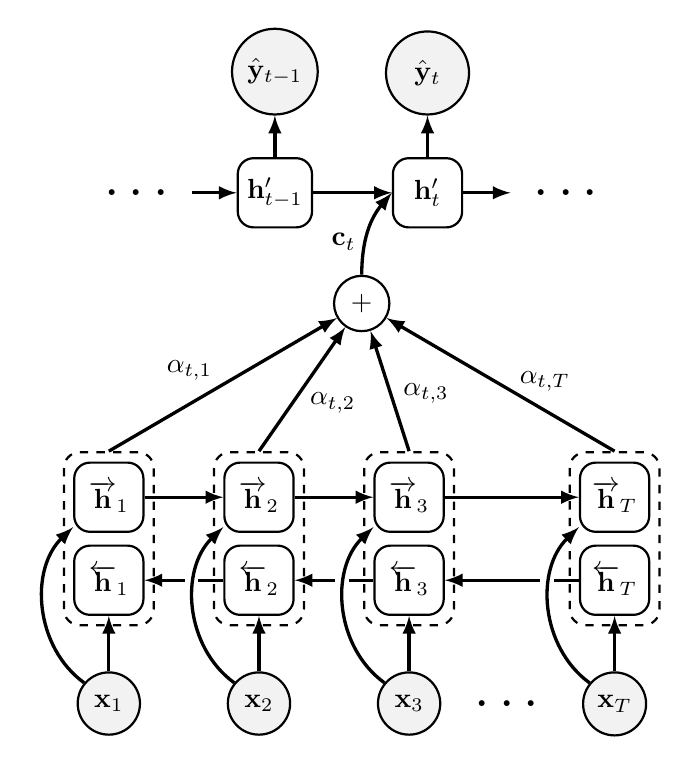
\begin{tikzpicture}[
    >=LaTeX, % Use default LaTeX arrows
    % Styles 
    cell/.style={ % RNN cell
        rectangle,
        rounded corners=2mm,
        minimum height=2.5em,
        minimum width=2.5em,
        draw,
        thick
    }, 
    cellc/.style={ % RNN cells in a chain
        cell,
        on chain,
        join
    },
    input/.style={ % Input or output node
        circle,
        minimum width=2.25em,
        draw,
        fill=gray!10,
        thick
    },
    op/.style={ % Summation node
        circle,
        draw,
        thick,
        minimum size=2em,
        inner sep=0pt
    },
    arrow/.style={
        -latex,
        very thick
    }
]

    % Forwards encoder RNN
    \begin{scope}[start chain=going right, nodes=cellc, arrow, local bounding box=chain]
        \path[shift={(-4em, 1em)}] 
            node (hb1) {$\overrightarrow{\mathbf{h}}_1$}
            node[] (hb2) {$\overrightarrow{\mathbf{h}}_2$} 
            node[] (hb3) {$\overrightarrow{\mathbf{h}}_3$} 
            node[xshift=2em] (hbT) {$\overrightarrow{\mathbf{h}}_{T}$};
    \end{scope}

    % Backwards encoder RNN
    \begin{scope}[start chain=going right, nodes=cellc, arrow, latex-, local bounding box=chain]
        \path[shift={(-4em, -2em)}] 
            node (h1) {$\overleftarrow{\mathbf{h}}_1$} 
            node[] (h2) {$\overleftarrow{\mathbf{h}}_2$} 
            node[] (h3) {$\overleftarrow{\mathbf{h}}_3$} 
            node[xshift=2em] (hT) {$\overleftarrow{\mathbf{h}}_{T}$};
    \end{scope}

    % Decoder RNN
    \begin{scope}[start chain=going right, nodes=cellc, arrow, local bounding box=chain]
        \path[shift={(2em, 12em)}] 
            node[] (h't-1) {$\mathbf{h}'_{t-1}$} 
            node[] (h't) {$\mathbf{h}'_{t}$};
    \end{scope}

    % Arrow from previous and arrow to next state in decoder
    \draw[arrow, latex-] (h't-1) -- ++ (-3em, 0);
    \draw[arrow] (h't) -- ++ (3em, 0);
    \node[scale=2] at ($(h't) + (5em, 0)$) {$\dots$};
    \node[scale=2] at ($(h't-1) + (-5em, 0)$) {$\dots$};

    % Summation
    \node[op] (sum) at ($(h1)!0.5!(hT) + (0, 10em)$) {$\mathbf{+}$};

    % Current context vector
    \draw[arrow, bend left=20] (sum.north) to node[pos=0.5, shift={(-0.9em, -0.4em)}] {$\mathbf{c}_t$} (h't.west);

    % Box surrounding corresponding cells in each RNN
    \foreach \X in {1, 2, 3, T} {
        \node[cell, dashed, fit=(hb\X) (h\X)] (box\X) {};
    }

    % Arrows from the top of the boxes to the summation node
    \draw[arrow] (box1.north) -- (sum) node[midway, left, shift={(0em,0.5em)}] {$\alpha_{t,1}$};
    \draw[arrow] (box2.north) -- (sum) node[midway, right, shift={(-0.1em,-0.5em)}] {$\alpha_{t,2}$};
    \draw[arrow] (box3.north) -- (sum) node[midway, right, shift={(0.1em,-0.1em)}] {$\alpha_{t,3}$};
    \draw[arrow] (boxT.north) -- (sum) node[midway, right, shift={(0.3em,0.1em)}] {$\alpha_{t,T}$};

    % White rectangles to create gaps between arrows
    \foreach \X in {1, 2, 3, T} {
        \fill[white] ($ (h\X.west) + (-0.9em,1em) $) rectangle ($ (h\X.west) + (-1.4em,-1em) $);
    }

    % Inputs and arrows from inputs
    \foreach \X in {1, 2, 3} {
        \draw[arrow, latex-] (h\X.south) -- ++ (0, -2em)
            node[below, input] (x\X) {$\mathbf{x}_\X$};
        \draw[arrow, latex-, bend right=50] (hb\X) to (x\X);
    }
    \draw[arrow, latex-] (hT.south) -- ++ (0, -2em)
        node[below, input] (xT) {$\mathbf{x}_{T}$};
    \draw[arrow, latex-, bend right=50] (hbT) to (xT);

    % Outputs and arrows to outputs
    \draw[arrow] (h't.north) -- ++ (0,1.5em)
        node[above, input, minimum width=3em] {$\hat{\mathbf{y}}_t$};
    \draw[arrow] (h't-1.north) -- ++ (0,1.5em)
        node[above, input, minimum width=3em] {$\hat{\mathbf{y}}_{t-1}$};
    
    % Continuation dots
    \path (x3) -- (xT) node[midway, scale=2] {\dots};

\end{tikzpicture}

\end{document}